\documentclass[10pt,twocolumn]{article}
\usepackage{tikz}
\usetikzlibrary{positioning, arrows.meta}
\usepackage{caption}

\begin{document}

\begin{figure*}[h!]
\centering
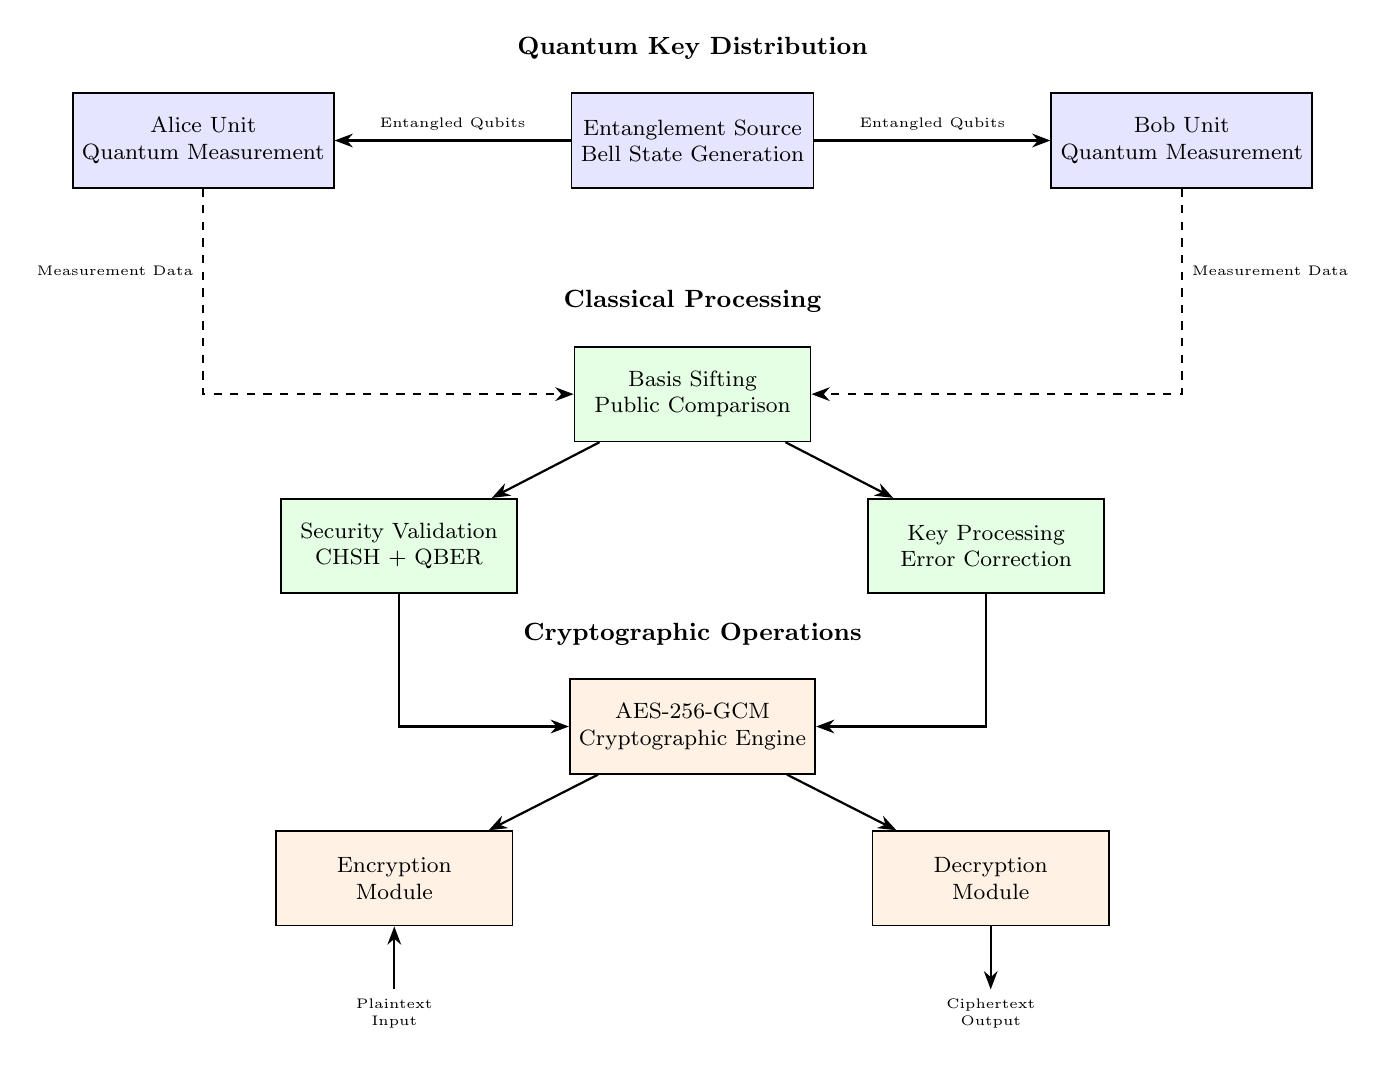
\begin{tikzpicture}[
    node distance=2cm and 3cm,
    every node/.style={font=\footnotesize},
    block/.style={
        rectangle,
        draw=black,
        fill=white,
        minimum width=3cm,
        minimum height=1.2cm,
        align=center,
        line width=0.6pt
    },
    quantum/.style={block, fill=blue!10},
    classical/.style={block, fill=green!10},
    crypto/.style={block, fill=orange!10},
    arrow/.style={
        -Stealth,
        line width=0.8pt,
        color=black
    }
]

% ==================== QUANTUM LAYER ====================
\node[quantum] (source) {Entanglement Source\\Bell State Generation};
\node[quantum, left=of source] (alice) {Alice Unit\\Quantum Measurement};
\node[quantum, right=of source] (bob) {Bob Unit\\Quantum Measurement};

% Quantum connections
\draw[arrow] (source) -- node[above, font=\tiny] {Entangled Qubits} (alice);
\draw[arrow] (source) -- node[above, font=\tiny] {Entangled Qubits} (bob);

% ==================== CLASSICAL PROCESSING LAYER ====================
\node[classical, below=2cm of source] (sifting) {Basis Sifting\\Public Comparison};
\node[classical, below left=1cm of sifting] (validation) {Security Validation\\CHSH + QBER};
\node[classical, below right=1cm of sifting] (keygen) {Key Processing\\Error Correction};

% Classical connections
\draw[arrow, dashed] (alice) |- node[pos=0.2, left, font=\tiny] {Measurement Data} (sifting);
\draw[arrow, dashed] (bob) |- node[pos=0.2, right, font=\tiny] {Measurement Data} (sifting);
\draw[arrow] (sifting) -- (validation);
\draw[arrow] (sifting) -- (keygen);

% ==================== CRYPTOGRAPHIC LAYER ====================
\node[crypto, below=3cm of sifting] (aes) {AES-256-GCM\\Cryptographic Engine};
\node[crypto, below left=1cm of aes] (encrypt) {Encryption\\Module};
\node[crypto, below right=1cm of aes] (decrypt) {Decryption\\Module};

% Crypto connections
\draw[arrow] (validation) |- (aes);
\draw[arrow] (keygen) |- (aes);
\draw[arrow] (aes) -- (encrypt);
\draw[arrow] (aes) -- (decrypt);

% ==================== DATA FLOW ====================
\node[below=0.8cm of encrypt, font=\tiny, align=center] (input) {Plaintext\\Input};
\node[below=0.8cm of decrypt, font=\tiny, align=center] (output) {Ciphertext\\Output};

\draw[arrow] (input) -- (encrypt);
\draw[arrow] (decrypt) -- (output);

% ==================== LAYER LABELS ====================
\node[above=0.3cm of source, font=\bfseries\small, align=center] {Quantum Key Distribution};
\node[above=0.3cm of sifting, font=\bfseries\small, align=center] {Classical Processing};
\node[above=0.3cm of aes, font=\bfseries\small, align=center] {Cryptographic Operations};

\end{tikzpicture}

\caption*{Figure: Architecture of the hybrid quantum classical cryptographic framework integrating QKD with AES-256-GCM encryption.}
\label{fig:qkd_aes_hybrid}
\end{figure*}

\end{document}